\documentclass{standalone}

\usepackage{pgfplots}
\usetikzlibrary{intersections}

\newcommand*{\ShowIntersectionWithSinAbs}{
\fill 
    [name intersections={of=DroiteK and SinAbs, name=i, total=\t}] 
    [red, opacity=1, every node/.style={above left, black, opacity=1}] 
    \foreach \s in {1,...,\t}{
        \ifodd \s 
        {}
        \else
        (i-\s) circle (2pt) node [above] {\s} 
        \fi 
        };
}
\newcommand*{\ShowIntersectionWithCosAbs}{
\fill 
    [name intersections={of=DroiteK and CosAbs, name=i, total=\t}] 
    [blue, opacity=1, every node/.style={above left, black, opacity=1}] 
    \foreach \s in {1,...,\t}{
        \ifodd \s 
        (i-\s) circle (2pt) node [above] {\s} 
        \fi 
        };
}
\newcommand*{\ShowIntersectionKfaibleWithCosAbs}{
\fill 
    [name intersections={of=DroiteKfaible and CosAbs, name=i, total=\t}] 
    [blue, opacity=1, every node/.style={above left, black, opacity=1}] 
    \foreach \s in {1,...,\t}{
        \ifodd \s 
        (i-\s) circle (1.3pt)  
        \fi 
        };
}
\newcommand*{\ShowIntersectionKfaibleWithSinAbs}{
\fill 
    [name intersections={of=DroiteKfaible and SinAbs, name=i, total=\t}] 
    [red, opacity=1, every node/.style={above left, black, opacity=1}] 
    \foreach \s in {1,...,\t}{
        \ifodd \s 
        (i-\s) circle (1.3pt)  
        \fi 
        };
}
\newcommand*{\ShowIntersectionKfortWithCosAbs}{
\fill 
    [name intersections={of=DroiteKfort and CosAbs, name=i, total=\t}] 
    [blue, opacity=1, every node/.style={above left, black, opacity=1}] 
    \foreach \s in {1,...,\t}{
        \ifodd \s 
        (i-\s) circle (1.3pt)  
        \fi 
        };
}
\newcommand*{\ShowIntersectionKfortWithSinAbs}{
\fill 
    [name intersections={of=DroiteKfort and SinAbs, name=i, total=\t}] 
    [red, opacity=1, every node/.style={above left, black, opacity=1}] 
    \foreach \s in {1,...,\t}{
        \ifodd \s 
        (i-\s) circle (1.3pt)  
        \fi 
        };
}
\begin{document}



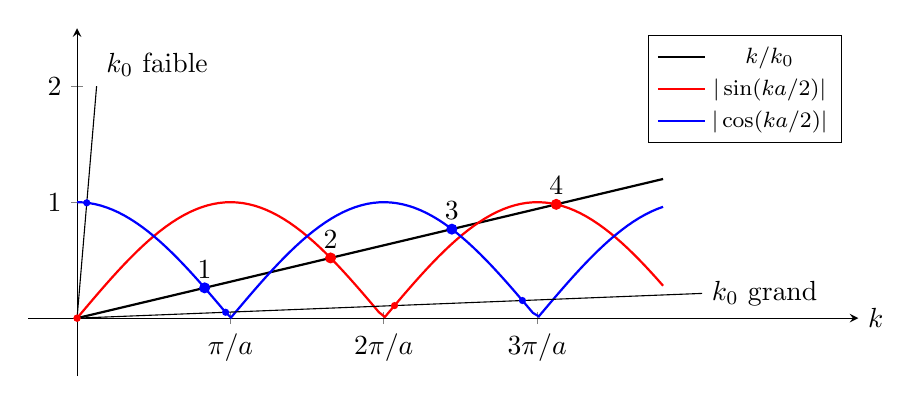
\begin{tikzpicture}
    \begin{axis}[
        xmax = 8,
        xmin = -0.5,
        ymin = -0.5,
        ymax = 2.5,
        axis lines = middle,
        xlabel style = {right},
        ylabel style = {above},
        xlabel = {$k$},
        width=\linewidth,
        height = 6cm,
        xtick = {1.57,3.14, {3.14+1.57}},
        xticklabels = {$\pi/a$,$2\pi/a$, $3\pi/a$},
        ytick = {},        
        ]
    
\addplot[name path global=DroiteK, mark=none, domain=0:6, thick]{x/5};%

\addplot [red, thick, name path global=SinAbs, domain = 0:6, samples = 100]  {abs(sin(deg(x)))} ;%

\addplot [blue, thick, name path global=CosAbs, domain = 0:6, samples = 100]  {abs(cos(deg(x)))};%


\addplot[name path global=DroiteKfaible, mark=none, domain=0:0.2]{x/0.1} node[anchor=south west] {$k_0$ faible};%
\addplot[name path global=DroiteKfort, mark=none, domain=0:6.4]{x/30} node[anchor=west]{$k_0$ grand};%


\ShowIntersectionWithSinAbs% Works
\ShowIntersectionWithCosAbs% Works
\ShowIntersectionKfaibleWithCosAbs
\ShowIntersectionKfaibleWithSinAbs
\ShowIntersectionKfortWithCosAbs
\ShowIntersectionKfortWithSinAbs

\legend{\footnotesize $k/k_0$, \footnotesize $|\sin(ka/2)|$, \footnotesize $|\cos(ka/2)|$}
\end{axis} 
\end{tikzpicture}
\end{document}